\section{What is CockroachDB?}
\emph{author: Felix Tröbinger}\bigskip

CockroachDB is advertised as a \enquote{cloud-native SQL database for building global, scalable cloud services that survive disasters}\cite{cockroach-github}. 

\medskip
CockroachDB is a relational and transactional database built for consistent key-value store and horizontal scalability and geo-replication as a big feature. It is built to ensure data survives failures of any kind, be that disk, machine rack or even entire datacenters.
Furthermore the database system is \enquote{strongly-consistent} and guarantees the ACID properites.\cite{cockroach-github} 

CockroachDB is considered a distributed database. It used geo-replication to ensure fast data access regardless of physical location. The distribution and geo-replication is presumably also what got the software its name.

\medskip
\emph{Cloud native}, often heard alongside \emph{microservices}, is a term that describes a system or a network of applications where single application, services or nodes are run inside Docker containers. 
Another important component in cloud-native computing is a load balancer, for example Kubernetes. 
CockroachDB is a good example of cloud-native computing since the Database is intended to be used in multiple locations and these multiple nodes are usually run in Docker containers. 

\subsection{History}
CockroachDB started as an open-source project in 2014.
Cockroach Labs was founded by ex-Google employees in the year 2015.\cite{cockroach-wired}
Spencer Kimball who is now CEO is also the original creator of the GNU Image Manipulation Program (GIMP).

\subsection{License and Pricing}
As stated above, CockroachDB was original an entirely open-source project and licensed under the second version of the Apache License (APL 2.0).
In 2019 however CockroachDB changed its license to a version of the Business Source License (BSL).
In summary, CockroachDB can still be used with as many nodes as desired except for offering a commercial cloud database system. 
CockroachDB Core is no longer open-source, however the source code can still be viewed on the companies GitHub page.
\cite{cockroach-license}

\medskip
Another interesting change in their license change is that versions of CockroachDB that are older than three years are converted to the APL. Although older versions (version 19.1 and downwards) are unaffected by this change and still use the Apache License as before. This is illustrated in figure \ref{fig:license}.

\begin{figure}[H]
    \caption{The new CockroachDB License model\cite{cockroach-license}}
    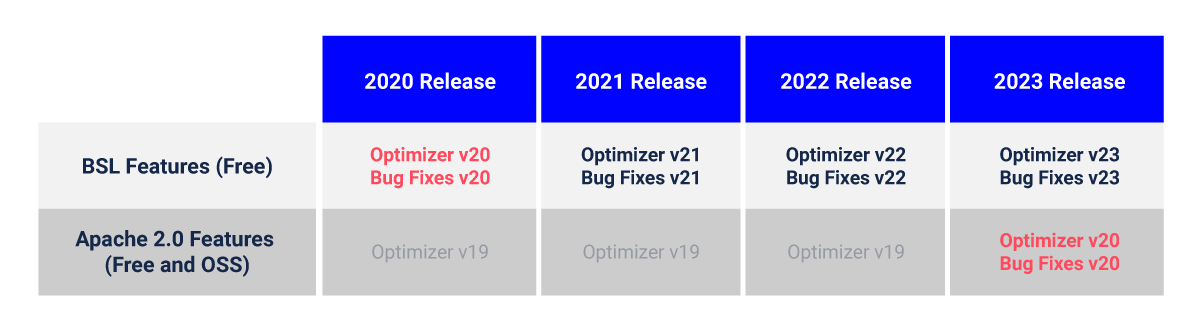
\includegraphics[width=\textwidth]{license}
    \label{fig:license}
\end{figure}


\bigskip
In terms of pricing, there are three available \enquote{Tiers} for CockroachDB:
\begin{itemize}
    \item \emph{CockroachCloud}
	\item \emph{CockroachEnterprise}
	\item \emph{CockroachDB Core}
\end{itemize}

\textbf{CockroachCloud} gives customers a fully hosted and managed database platform. 
The price for this service is calculated per node and hour and differs depending on whether the customer chooses AWS (Amazon Web Services) or Google Cloud as a hosting platform.
The price also changes depending on the CPU power and hard drive size of the node.
\cite{cockroach-pricing}

\medskip
The mayor differences to the \textbf{CockroachDB Enterprise} tier is that this option gives the customer superior support and that it is self hosted, meaning that the customer does not rely on Cockroach Labs to store their data, but will rather host it themselves. This means that the customer has to pay another company to do that for them or take it on their own to host CockroachDB nodes in a distributed manner.
As for price, Cockroach Labs invite customers to contact them.
\cite{cockroach-pricing}

\medskip
On the CockroachDB page for pricing the company states that \textbf{CockroachDB Core} is open-source,\cite{cockroach-pricing} yet an article covering the licensing of the product explains that this version of the database is not actually open-source according to OSI’s Open Source Definition (though the source code is still viewable to anyone).\cite{cockroach-license}
This version however is free to download and use. 



